
\documentclass[%
pdftex,
oneside,			% Einseitiger Druck.
11pt,				% Schriftgroesse
parskip=half,		% Halbe Zeile Abstand zwischen Absätzen.
%	topmargin = 10pt,	% Abstand Seitenrand (Std:1in) zu Kopfzeile [laut log: unused]
headheight = 12pt,	% Höhe der Kopfzeile
%	headsep = 30pt,	% Abstand zwischen Kopfzeile und Text Body  [laut log: unused]
headsepline,		% Linie nach Kopfzeile.
footsepline,		% Linie vor Fusszeile.
footheight = 16pt,	% Höhe der Fusszeile
abstracton,		% Abstract Überschriften
DIV=calc,		% Satzspiegel berechnen
BCOR=8mm,		% Bindekorrektur links: 8mm
headinclude=false,	% Kopfzeile nicht in den Satzspiegel einbeziehen
footinclude=false,	% Fußzeile nicht in den Satzspiegel einbeziehen
listof=totoc,		% Abbildungs-/ Tabellenverzeichnis im Inhaltsverzeichnis darstellen
toc=bibliography,	% Literaturverzeichnis im Inhaltsverzeichnis darstellen
]{scrreprt}	% Koma-Script report-Klasse, fuer laengere Bachelorarbeiten alternativ auch: scrbook

%To-Do: Felder bei Abgabe wieder richtig setzen

\def \titel {Automatisierung des Bereitschaftsdienstplans für Einsatzfahrende mithilfe eines Vorhersagemodells} 
\def \arbeit {Fallstudie}
\def \autor {<to be replaced>}%{Jasper Bremenkamp}
\def \abschluss {<to be replaced>}%{M.Sc.}
\def \studiengang {<to be replaced>}%{Data Science}
\def \datumAbgabe {<to be replaced>}%{\today}
\def \modul {<to be replaced>}%{Model Engineering}
\def \matrikelnr {<to be replaced>}%{92125193}
\def \tutor {<to be replaced>}%{Markus Pak}

\def \seitenrand {2cm}

% PDF Einstellungen
\usepackage{hyperref}

\hypersetup{ 
    unicode = true,
    pdftitle={\titel},
    pdfauthor={\autor},
    pdfsubject={\arbeit},
    pdfcreator={pdflatex, LaTeX with KOMA-Script},
    pdfpagemode=UseOutlines,    % Beim Oeffnen Inhaltsverzeichnis anzeigen
    pdfdisplaydoctitle=true,    % Dokumenttitel statt Dateiname anzeigen.
    pdflang={de},   % Sprache des Dokuments.
    hidelinks
}

\usepackage[left=2cm,right=2cm,top=2cm,bottom=2cm]{geometry} % margins	% Seitenränder und Abstände
\usepackage[activate]{microtype} %Zeilenumbruch und mehr
\usepackage[onehalfspacing]{setspace}
\usepackage{makeidx}
\usepackage[autostyle=true,german=quotes]{csquotes}
\MakeOuterQuote{"} % Für deutsche Anführungszeichen 
\usepackage{longtable}
\usepackage{enumitem}	% mehr Optionen bei Aufzählungen
\usepackage{graphicx}
\usepackage{pdfpages}   % zum Einbinden von PDFs
\usepackage{xcolor} 	% für HTML-Notation
\usepackage{float}
\usepackage{array}
\usepackage{calc}		% zum Rechnen (Bildtabelle in Deckblatt)
\usepackage[right]{eurosym}
\usepackage{wrapfig}
\usepackage{pgffor} % für automatische Kapiteldateieinbindung
\usepackage[perpage, hang, multiple, stable]{footmisc} % Fussnoten
\usepackage[printonlyused]{acronym} % falls gewünscht kann die Option footnote eingefügt werden, dann wird die Erklärung nicht inline sondern in einer Fußnote dargestellt
\usepackage{listings}
\usepackage{bookmark}
\usepackage[english, ngerman]{babel}
\usepackage[utf8]{inputenc}
\usepackage{scrhack}
\usepackage[T1]{fontenc} %Damit Umlaute auch beim Kopieren richtig dargestellt werden
\usepackage{caption} %für captionof
\usepackage{graphicx}
\usepackage{placeins}
\usepackage{dirtree}
\usepackage{booktabs}
\usepackage{makecell}

    %%%%%%% Neues Design %%%%%%%%%%%

    \usepackage{helvet} %Arial-Ersatz
    \renewcommand{\familydefault}{\sfdefault}
    
    \def\UrlFont{\rm} % Print URLs not in Typewriter Font

    \usepackage{etoolbox}
    \makeatletter
    \patchcmd{\scr@startchapter}{\if@openright\cleardoublepage\else\clearpage\fi}{}{}{} %entfernt das starten einer neuen Seite bei einem neuen Chapter
    \makeatother

    %\addtolength{\footskip}{-0.7cm}% foot larger by 0,7 cm  (Raises the page number)
    %\setlength{\parindent}{6pt} % Indent at start of paragraphs  6pt

    \usepackage{titlesec} % define size for section headings
    \titleformat{\chapter}{\normalfont\fontsize{12pt}{1.5}\bfseries}{\thechapter}{1em}{}
    \titleformat{\section}{\normalfont\fontsize{12pt}{1.5}\bfseries}{\thesection}{1em}{}
    \titleformat{\subsection}{\normalfont\fontsize{12pt}{1.5}\bfseries}{\thesubsection}{1em}{} 

    \renewcommand{\footnotesize}{\fontsize{10pt}{1.5pt}\selectfont}

    \titlespacing{\chapter}{0pt}{10pt}{10pt}

    %%%%%%%%%%%%%%%%%%%%%%%%%%%%%%%

% Notizen. Einsatz mit \todo{Notiz} oder \todo[inline]{Notiz}. 
\usepackage[obeyFinal,backgroundcolor=yellow,linecolor=black]{todonotes}
% Alle Notizen ausblenden mit der Option "final" in \documentclass[...] oder durch das auskommentieren folgender Zeile
% \usepackage[disable]{todonotes}

% Kommentarumgebung. Einsatz mit \comment{}. Alle Kommentare ausblenden mit dem Auskommentieren der folgenden und dem aktivieren der nächsten Zeile.
\newcommand{\comment}[1]{\par {\bfseries \color{blue} #1 \par}} %Kommentar anzeigen

% der neue Zitierstil ist Käse
\global\def\VAlterZitierstil{true}

\global\def\VTrueValue{true}

\ifx\VAlterZitierstil\VTrueValue
    % \usepackage[
    %     backend=biber,     % biber muss seperat installiert werden
    %     bibwarn=true,
    %     bibencoding=utf8,   % wenn .bib in utf8, sonst ascii
    %     sortlocale=de_DE,
    %     sorting=none,
    %     style=apa %apa instead of IEEE
    % ]{biblatex}

    \usepackage[backend=biber, style=apa, pagetracker, ibidtracker=constrict, apamaxprtauth=20 ]{biblatex}

    %Enable IBAN on APA style
    \usepackage{xpatch}
    \xpretobibmacro{doi+url}{\printfield{isbn}}{}{}

    \addbibresource{bibliographie.bib}
\else
    %eigentlich totaler Käse, kann nach Bewertung der Arbeit für zukünftige Arbeiten entfernt werden

    % New IUBH Cite Style / Old Cite style over this block
    % \usepackage{natbib}
    % \setcitestyle{aysep={}} % remove comma as delimiter 

    \usepackage{apacite}

    %search and replace von apacite zur biblatex
    %Search: \\citeNP<([^}]*)>\[([^}]*)\]\{([^}]+)\}
    %Replace: \\cite[$1][$2]{$3}
\fi

\definecolor{codegreen}{rgb}{0,0.6,0}
\definecolor{codegray}{rgb}{0.5,0.5,0.5}
\definecolor{codepurple}{rgb}{0.58,0,0.82}
\definecolor{backcolour}{rgb}{0.95,0.95,0.92}

\lstdefinestyle{mystyle}{
    backgroundcolor=\color{backcolour},
    commentstyle=\color{codegreen},
    keywordstyle=\color{magenta},
    numberstyle=\tiny\color{codegray},
    stringstyle=\color{codepurple},
    basicstyle=\ttfamily\footnotesize,
    breakatwhitespace=false,
    breaklines=true, 
    captionpos=b,
    keepspaces=true,
    numbers=left,
    numbersep=5pt,
    showspaces=false,
    showstringspaces=false,
    showtabs=false,
    tabsize=2
}

\lstdefinestyle{yaml}{
     basicstyle=\color{blue}\footnotesize,
     rulecolor=\color{black},
     string=[s]{'}{'},
     stringstyle=\color{blue},
     comment=[l]{:},
     commentstyle=\color{black},
     morecomment=[l]{-}
 }

\lstset{style=mystyle}

\renewcommand{\lstlistingname}{Code Ausschnitt}% 
\renewcommand{\lstlistlistingname}{Code-Ausschnitt-Verzeichnis}%

\begin{document}

\pagenumbering{Roman}

\begin{titlepage}
    \begin{figure}[h]
        \centering
        \advance\leftskip--2cm
        %
\includegraphics[width=0.50\textwidth]{assets/logo.pdf} %To-Do: wieder einbauen
        \end{figure}
        \FloatBarrier
        
        \begin{Large} 
        \begin{center}
        \arbeit
        \end{center}
        \end{Large} 
        
        \vspace*{30mm}
        
        \begin{Large} 
        \begin{center}
        \textbf{\titel}
        \end{center}
        \end{Large}
        
        \vspace*{45mm}
        
        \begin{large} 
        \begin{center}
        \autor
        \end{center}
        \end{large} 
        
        \vspace*{-6mm}
        
        \begin{large} 
        \begin{center}
        Matrikelnummer: \matrikelnr
        \end{center}
        \end{large} 
        
        \vspace*{-6mm}
        
        \begin{large} 
        \begin{center}
        % ursprünglich Straße
        \end{center}
        \end{large} 
        
        \vspace*{24mm}
        
        \begin{large} 
        \begin{center}
        erfolgt im Kurs \enquote{\modul} \\
        des Studiengangs \abschluss { }\studiengang
        \end{center}
        \end{large} 
        
        \vspace*{10mm}
        
        \begin{large} 
        \begin{center}
        Tutor: \tutor 
        \end{center}
        \end{large}         
        \vspace*{-6mm}
        
        \begin{large} 
        \begin{center}
        Abgabedatum: \datumAbgabe
        \end{center}
        \end{large} 
\end{titlepage}

\renewcommand{\abstractname}{Abstract}
\begin{abstract}

    % Zum Schluss nochmal neuschreiben bzw. überarbeiten

    In dieser Arbeit wird die Automatisierung des Bereitschaftsdienstplans für Einsatzfahrende mithilfe eines Vorhersagemodells untersucht. 
    Der Prozess umfasst eine detaillierte Datenanalyse, die auf einem bereitgestellten CSV-Datensatz basiert, welcher Informationen über krankheitsbedingte Abwesenheiten und Anrufvolumina enthält. 
    Die Analyse umfasst die explorative Datenanalyse (EDA), Datenbereinigung und -vorbereitung sowie die Erstellung eines Basismodells und eines präziseren Vorhersagemodells.

    Zunächst wird der Datensatz inspiziert und grundlegende Statistiken sowie Visualisierungen zur Verteilung der Variablen n\_sick (Anzahl der erkrankten Mitarbeiter) und calls (Anrufvolumen) erstellt. 
    Dabei wird die zeitliche Dimension berücksichtigt, um saisonale Trends und Muster zu erkennen. 
    Die Datenvorbereitung beinhaltet die Behandlung fehlender Werte, Feature Engineering und die Aufteilung in Trainings- und Testdatensätze.
    
    Ein Basismodell wird als Ausgangspunkt implementiert und seine Leistung mittels Mean Absolute Error (MAE) bewertet.
    Anschließend wird ein fortgeschritteneres Modell (Random Forest) trainiert und durch Hyperparameter-Tuning optimiert. 
    Die Modelle werden anhand von MAE und Feature-Importance-Analysen evaluiert, um die wichtigsten Einflussfaktoren zu identifizieren.
    
    Die Ergebnisse der Datenanalyse und Modellierung werden durch geeignete Visualisierungen und Berichte kommuniziert. 
    Dies ermöglicht eine fundierte Entscheidungsfindung und trägt zur Effizienzsteigerung des Bereitschaftsdienstplans bei, indem präzisere Vorhersagen über krankheitsbedingte Abwesenheiten getroffen werden können. 
    Die Arbeit zeigt, dass eine strukturierte Vorgehensweise bei der Datenanalyse und Modellierung wesentliche Erkenntnisse liefert, die zur Optimierung betrieblicher Prozesse beitragen.
    

\end{abstract}

% Inhaltsverzeichnis
\begin{spacing}{1.1}
    \begingroup
    
        % auskommentieren für Seitenzahlen unter Inhaltsverzeichnis
        \renewcommand*{\chapterpagestyle}{empty}
        \pagestyle{empty}

        \setcounter{tocdepth}{3}
        %für die Anzeige von Unterkapiteln im Inhaltsverzeichnis
        %\setcounter{tocdepth}{2}
        
        \tableofcontents
        \clearpage
    \endgroup
\end{spacing}
\newpage

%Abbildungsverzeichnis
\cleardoublepage 
\listoffigures
\clearpage

\lstlistoflistings %List of listings
\clearpage

%Tabellenverzeichnis
%\cleardoublepage
%\listoftables

\chapter{Einleitung}
\pagenumbering{arabic}

    % Ziel: Einleitung: ca. 20%
    % Dafür wären eigentlich 2,5 Seiten nötig! Evtl strecken oder Bilder einbauen!

    Die effiziente Planung des Bereitschaftsdienstes für Einsatzfahrende stellt den Berliner Rotkreuz-Rettungsdienst vor erhebliche Herausforderungen. 
    Die derzeitige Planungslogik erweist sich als unzureichend, insbesondere bei kurzfristigen Krankenständen und unvorhersehbar hohen Notrufaufkommen. 
    (\cite[Vgl.][S. 3, 4]{data_science_aufgabenstellung})

    Diese unvorhersehbaren Ereignisse führen regelmäßig zu Kapazitätsengpässen, die nur durch die kurzfristige Aktivierung zusätzlicher Einsatzfahrender ausgeglichen werden können. 
    Solche ad-hoc Lösungen sind jedoch oft ineffizient und können die Einsatzbereitschaft und Reaktionszeit negativ beeinflussen.

    Das Ziel dieses Projekts ist es, die bestehende Planungslogik zu verbessern und die Bereitschaftsdienstplanung zu automatisieren. 
    Mithilfe eines Vorhersagemodells soll die Anzahl der erforderlichen Einsatzfahrenden im Bereitschaftsdienst auf Tagesbasis effizient abgeschätzt werden. %To-Do: Verifizieren was genau vorhersagt werden muss und ggf hier anpassen. Anzahl der Kranken (n_suck). Anzahl der Einsätze (?), Anzahl der benötigten Bereitschaftsdiensthabenden (sby_need)?
    Ein besonderes Augenmerk liegt dabei auf der Identifikation saisonaler Muster, wie zum Beispiel die erhöhte Ausfallrate in den Wintermonaten. 
    Durch die Analyse historischer Daten zu Abwesenheiten und Notrufaufkommen sollen präzise Vorhersagen getroffen werden, um die Einsatzbereitschaft optimal zu gewährleisten.
    (\cite[Vgl.][S. 3, 4]{data_science_aufgabenstellung})
    
    Ein datengetriebener Ansatz bietet hier signifikante Vorteile. 
    Durch die Nutzung von maschinellem Lernen können komplexe Muster und Zusammenhänge in den Daten erkannt werden, die mit herkömmlichen Methoden schwer zu identifizieren wären. 
    Dies ermöglicht eine proaktive und vorausschauende Planung, die sowohl die Zufriedenheit der Einsatzfahrenden als auch die Effizienz des Rettungsdienstes verbessert.
    
    Das Vorhersagemodell wird darauf abzielen, den Prozentsatz der aktivierten Einsatzfahrenden zu maximieren und die Tage mit zu wenigen Einsatzfahrenden zu minimieren. 
    Ziel ist es mindestens 90\% aktive Bereitschaftsfahrende pro Tag zu haben und die Extrakapazitäten noch vor Ende des 15. vom Folgemonat eingeplant zu haben.
    Dies soll zu einer besseren Planbarkeit und einer effizienteren Ressourcennutzung führen. 
    Ein weiterer wichtiger Aspekt ist die Benutzerfreundlichkeit des Systems. 
    Das Modell soll in eine intuitive Benutzeroberfläche integriert werden, die den Planungsverantwortlichen die Handhabung erleichtert und ihnen erlaubt, schnell und flexibel auf Veränderungen zu reagieren.
    
    In den folgenden Kapiteln wird das Projekt im Detail beschrieben. 
    Zunächst wird die angewendete Projektmanagementmethodik erläutert und die Strukturierung des Git-Repositories vorgestellt. 
    Daraufhin folgt eine ausführliche Datenanalyse, die die Grundlage für die Modellierung bildet. 
    Es werden sowohl ein erstes Basismodell als auch ein präziseres Vorhersagemodell entwickelt und deren Performance evaluiert. 
    Besonderes Augenmerk wird dabei auf die Interpretierbarkeit der Modellresultate und eine detaillierte Fehleranalyse gelegt. 
    Abschließend wird ein Vorschlag zur Integration des Modells in den Arbeitsalltag des Fachbereichs präsentiert und eine beispielhafte grafische Benutzeroberfläche vorgestellt. 
    Die Arbeit schließt mit einer Zusammenfassung der Ergebnisse und Empfehlungen für zukünftige Arbeiten oder Verbesserungen.
    
    Durch die erfolgreiche Implementierung dieses Projekts könnte der Berliner Rotkreuz-Rettungsdienst einen bedeutenden Schritt in Richtung einer moderneren und effizienteren Bereitschaftsdienstplanung machen. 
    Dies würde nicht nur die Einsatzbereitschaft und Reaktionszeit verbessern, sondern auch die Arbeitszufriedenheit der Einsatzfahrenden erhöhen.
    

\chapter{Projektmanagement und Methodik}

    Die erfolgreiche Umsetzung eines datengetriebenen Projekts wie der Automatisierung des Bereitschaftsdienstplans erfordert eine strukturierte und systematische Vorgehensweise. 
    In diesem Kapitel werden die angewendete Projektmanagementmethodik und die vorgeschlagene Ordnerstruktur des Git-Repositories beschrieben.

    \section{Projektmanagementmethodik}

        Für dieses Projekt wird die CRISP-DM (Cross Industry Standard Process for Data Mining) Methodik verwendet, die sich als Industriestandard für Data-Mining-Projekte etabliert hat. 
        Die Wahl von CRISP-DM gegenüber der Microsoft Team Data Science Process (TDSP) Methode wurde aus mehreren Gründen getroffen:

        % To-Do bei Platzmangel diesen Stichpunkt Block kürzen oder gänzlich ersetzen
        \begin{itemize}
            \item \textbf{Reife und Anerkennung}: CRISP-DM ist seit den 1990er Jahren etabliert und hat sich als Industriestandard bewährt. 
            Es ist gut dokumentiert und wird in verschiedenen Branchen erfolgreich angewendet.
            \item \textbf{Universelle Anwendbarkeit}: CRISP-DM ist technologie- und plattformunabhängig und kann in einer Vielzahl von Projekten und mit unterschiedlichen Toolsets genutzt werden. 
            Dies macht es besonders flexibel für Projekte, die hybride Umgebungen nutzen.
            \item \textbf{Klare Phasenstruktur}: CRISP-DM besteht aus sechs klar definierten Phasen (Business Understanding, Data Understanding, Data Preparation, Modeling, Evaluation, Deployment), die einen systematischen und leicht nachvollziehbaren Ablauf bieten.
            \item \textbf{Umfangreiche Ressourcen}: Es gibt eine Fülle an Ressourcen, Fallstudien, Best Practices und Community-Support für CRISP-DM, was den Einstieg erleichtert und die Wahrscheinlichkeit eines erfolgreichen Projekts erhöht.
            \item \textbf{Erfahrung und Vertrautheit}: Viele Data-Science-Teams und Fachleute sind bereits mit CRISP-DM vertraut, was den Schulungsaufwand reduziert und die Implementierung beschleunigt.
        \end{itemize}
        (\cite[Vgl.][]{crisp_vs_tdsp}) %To-Do: prüfen, ob es sich mit Inhalt ausreichen viel überschneidet

        Die CRISP-DM Methodik umfasst die folgenden sechs Phasen:

        \begin{enumerate}
            \item \textbf{Business Understanding}: In dieser Phase wird das Geschäftsproblem definiert, die Ziele des Projekts festgelegt und die Anforderungen spezifiziert. 
            Für unser Projekt bedeutet dies, die Herausforderungen der aktuellen Bereitschaftsdienstplanung zu verstehen und die Zielsetzungen der Automatisierung klar zu formulieren.
            \item \textbf{Data Understanding}: Diese Phase beinhaltet das Sammeln von Daten, die erste Datenexploration und die Bewertung der Datenqualität. 
            Im Rahmen dieses Projekts werden historische Daten zu Abwesenheiten und Notrufaufkommen analysiert.
            \item \textbf{Data Preparation}: Hier werden die Daten bereinigt und transformiert, um sie für die Modellierung vorzubereiten. 
            Dies umfasst das Handling fehlender Werte, die Erstellung neuer Features und die Skalierung der Daten.
            \item \textbf{Modeling}: In dieser Phase werden verschiedene Modellierungstechniken angewendet und optimiert. 
            Ein Basismodell wird entwickelt und anschließend durch ein präziseres Vorhersagemodell ersetzt.
            \item \textbf{Evaluation}: Die Modellleistung wird anhand relevanter Metriken bewertet und überprüft, ob die Modellziele erreicht wurden. 
            Dies beinhaltet auch eine Fehleranalyse und die Interpretation der Modellresultate.
            \item \textbf{Deployment}: Schließlich wird das Modell in den operativen Betrieb integriert. 
            Dies umfasst die Implementierung in eine graphische Benutzeroberfläche und die Schulung der Nutzer.
        \end{enumerate}
        (\cite[Vgl.][S. 14]{shearer2000crisp})

        CRISP-DM bietet eine klare, phasenbasierte Struktur bietet, die sich gut für klassische Data-Science-Projekte eignet.
        TDSP stärker auf moderne, agile Praktiken und die Integration in bestehende Systeme fokussiert und würde daher stärker auf Iterationen, Automatisierung und die Einbindung von DevOps-Praktiken ausgerichtet sein.
        Für die Dokumentstruktur und den Ablauf ist CRISP-DM auch deshalb die bessere Wahl und dessen Phasen finden sich im ganzen Dokument wieder.

    \section{Struktur des Git-Repositories}

        Ein gut strukturiertes Git-Repository ist entscheidend für die effiziente Zusammenarbeit im Projektteam und die Nachvollziehbarkeit der Entwicklungsschritte. 
        Die folgende Ordnerstruktur wird für dieses Projekt vorgeschlagen:

        % To-do Zum Schluss, Richtung Abgabe die Struktur an den Ist-Zustand anpassen 
        \dirtree{%
        .1 /.
        .2 data.
        .3 raw.
        .3 processed.
        .2 notebooks.
        .3 exploration.
        .3 modeling.
        .2 app. 
        .3 data\_preparation.
        .3 models.
        .3 evaluation.
        .2 reports.
        .3 figures.
        .3 tables.
        .2 docs.
        }

        \begin{itemize}
            \item \textbf{data}: Dieser Ordner enthält alle Daten, die im Projekt verwendet werden. 
            Der Unterordner \textit{raw} speichert die unbearbeiteten Rohdaten, während im Unterordner \textit{processed} die für die Modellierung vorbereiteten Daten abgelegt werden.
            \item \textbf{notebooks}: Hier werden Jupyter-Notebooks für die Datenexploration und Modellierung gespeichert. 
            Der Unterordner \textit{exploration} enthält Notebooks zur ersten Datenanalyse, und der Unterordner \textit{modeling} enthält Notebooks zur Entwicklung und Evaluation der Modelle.
            \item \textbf{app}: In diesem Ordner sind die Skripte zur Datenvorbereitung, Modellierung und Evaluation gespeichert. %To-Do: Aktuell halten
            Die Skripte im Unterordner \textit{data\_preparation} kümmern sich um die Datenbereinigung und -transformation, während im Unterordner \textit{models} die Modelltrainingsskripte und im Unterordner \textit{evaluation} die Evaluationsskripte abgelegt werden.
            \item \textbf{reports}: Dieser Ordner enthält alle Berichte, Abbildungen und Tabellen, die im Laufe des Projekts erstellt werden. 
            Der Unterordner \textit{figures} speichert Grafiken und Diagramme, während der Unterordner \textit{tables} die erstellten Tabellen enthält.
            \item \textbf{docs}: Hier werden alle Projektdokumentationen abgelegt. 
            Dies umfasst Projektpläne, Anforderungsdokumente und andere relevante Dokumente.
        \end{itemize}

        Diese strukturierte Vorgehensweise und die klare Organisation des Repositories tragen wesentlich zur Effizienz und Transparenz des Projekts bei und erleichtern die Zusammenarbeit im Team.

\chapter{Datenanalyse}
        
        Die Datenanalyse ist ein wesentlicher Bestandteil des Projekts, da sie die Grundlage für die Entwicklung und Optimierung des Vorhersagemodells bildet. 
        Das Vorgehen zur Datenanalyse gliedert sich in mehrere Schritte, die im Folgenden detailliert beschrieben werden.

    \section{Explorative Datenanalyse (EDA)}

        Die explorative Datenanalyse (EDA) bildet die Grundlage für das Verständnis der bereitgestellten Daten und die Identifikation von Mustern und Zusammenhängen. 
        Für dieses Projekt wurden die Daten in mehreren Schritten untersucht und analysiert.

        \subsection{Dateninspektion}

            Zunächst wurden die Daten auf ihre Grundstruktur hin untersucht. 
            Dabei wurden Informationen wie die Anzahl der Datensätze, die Struktur der Datensätze und das Vorhandensein von fehlenden Werten erfasst. 
            Die wichtigsten Merkmale der Daten sind in Tabelle \ref{tab:data_summary} zusammengefasst.

            \begin{table}[H]
                \centering
                \begin{tabular}{|l|l|}
                \hline
                \textbf{Merkmal} & \textbf{Beschreibung} \\ \hline
                date & Datum des Eintrags \\ \hline
                n\_sick & Anzahl der Einsatzfahrer, die einen Krankenstand angemeldet haben \\ \hline
                calls & Anzahl der Notrufe \\ \hline
                n\_duty & Anzahl der Einsatzfahrer im Dienst \\ \hline
                n\_sby & Anzahl der verfügbaren Ersatzfahrer \\ \hline
                sby\_need &  Anzahl der Ersatzfahrer, die aktiviert werden \\ \hline
                drafted & \makecell{Anzahl der zusätzlichen Einsatzfahrer, die aktiviert werden müssen,\\ wenn die Anzahl der Einsatzfahrer im Bereitschaftsdienst nicht ausreicht} \\ \hline
                \end{tabular}
                \\
                (\cite[Vgl.][S. 2, 3]{data_science_aufgabenstellung_zusatz})
                \caption{Zusammenfassung der Datensätze}
                \label{tab:data_summary}
            \end{table}


        \subsection{Verteilung der Merkmale}

            Die Verteilungen der wichtigsten Merkmale wurden mittels Histogrammen und Dichteplots visualisiert. 
            Diese Visualisierungen halfen dabei, die Verteilung der Daten und das Vorhandensein von Ausreißern zu verstehen. 
            Abbildungen \ref{fig:n_sick_dist} und \ref{fig:calls_dist} zeigen die Verteilungen der Merkmale \textit{n\_sick} und \textit{calls}.

            \begin{figure}[H]
                \centering
                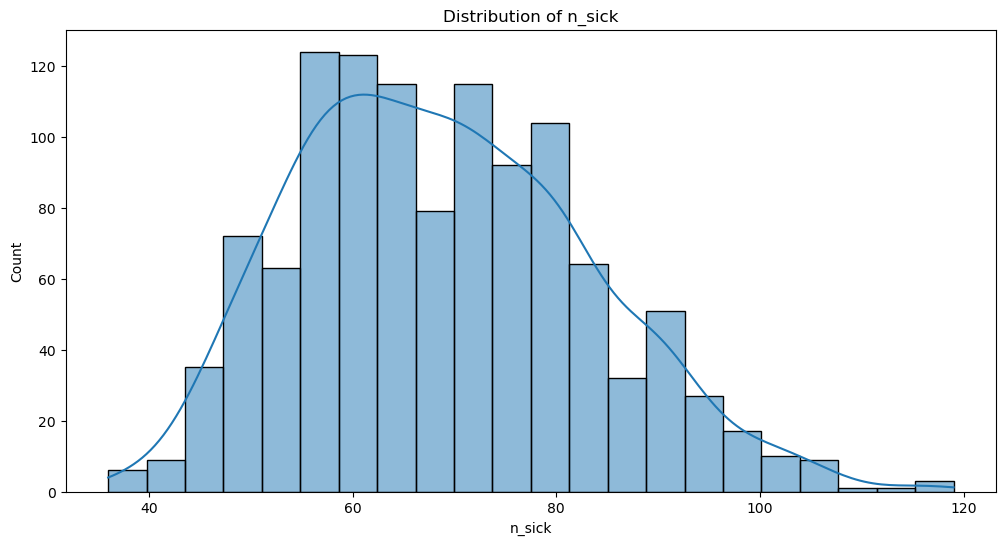
\includegraphics[width=0.8\textwidth]{assets/n_sick_dist.png}
                \caption{Verteilung der Anzahl der Krankmeldungen (n\_sick)}
                \label{fig:n_sick_dist}
            \end{figure}

            \begin{figure}[H]
                \centering
                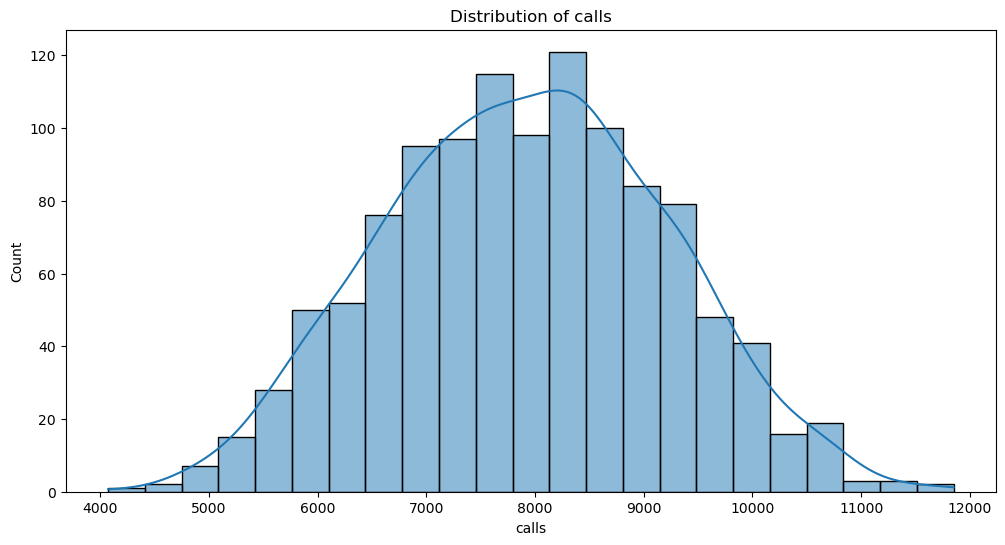
\includegraphics[width=0.8\textwidth]{assets/calls_dist.png}
                \caption{Verteilung der Anzahl der Anrufe (calls)}
                \label{fig:calls_dist}
            \end{figure}

        \subsection{Korrelationen}

            Die Korrelationen zwischen den verschiedenen Merkmalen wurden mittels einer Korrelationsmatrix untersucht. 
            Abbildung \ref{fig:corr_matrix} zeigt die Korrelationsmatrix der Merkmale.

            \begin{figure}[H]
                \centering
                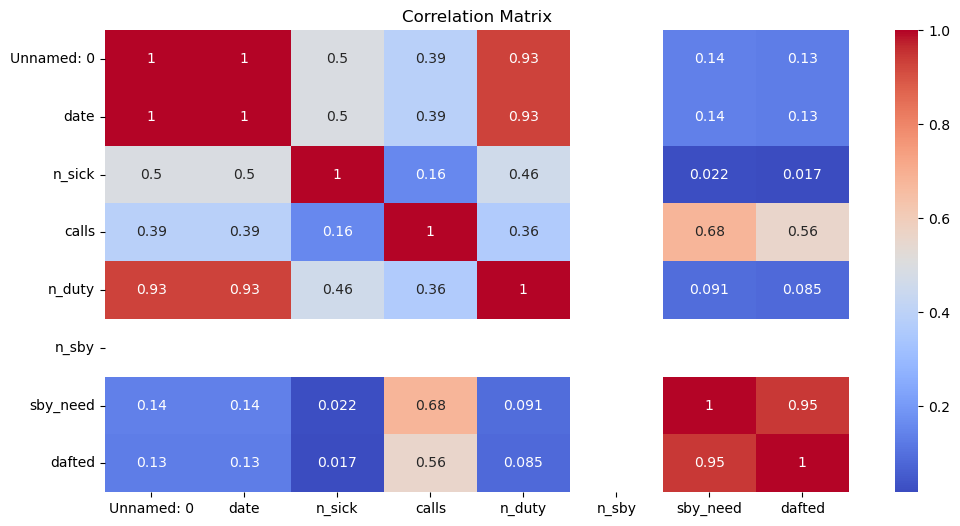
\includegraphics[width=0.8\textwidth]{assets/corr_matrix.png}
                \caption{Korrelationsmatrix der Merkmale}
                \label{fig:corr_matrix}
            \end{figure}

    \section{Datenvorbereitung}

        Nach der initialen Untersuchung und Analyse der Daten wird die Datenvorbereitung durchgeführt. 
        Dieser Schritt ist entscheidend, um die Daten in ein Format zu bringen, das für die Modellierung geeignet ist.

        \subsection{Umgang mit fehlenden Werten}

            %To-Do: Nochmal zum Schluss prüfen, ob das hier passt

            Fehlende Werte liegen nicht vor.
            Falls dennoch welche wären, würden sie entfernt, um die Integrität der Daten zu gewährleisten.

        \subsection{Feature Engineering}

            Ein wichtiger Teil der Datenvorbereitung ist das Feature Engineering. 
            Hierbei werden neue Merkmale erstellt, die das Vorhersagemodell verbessern können. 
            Basierend auf den Erkenntnissen der EDA werden zeitliche Merkmale wie der Monat und der Wochentag aus dem Datum extrahiert. 
            Tabelle \ref{tab:new_features} zeigt die neuen Merkmale, die erstellt wurden.

            \begin{table}[H]
                \centering
                \begin{tabular}{|l|l|}
                \hline
                \textbf{Neues Merkmal} & \textbf{Beschreibung} \\ \hline
                month & Monat des Jahres \\ \hline
                day\_of\_week & Wochentag \\ \hline
                \end{tabular}
                \caption{Erstellte neue Merkmale}
                \label{tab:new_features}
            \end{table}

        \subsection{Datenaufteilung}

            % Auf Zeitform achten. Wann Vergangenheit und wann Zukunft?
            % Hier noch Zukunft, da bis hier ja noch nicht umgesetzt.

            Für die Modellierung werden die Daten in Trainings- und Testdaten aufgeteilt. 
            Dies ermöglicht eine objektive Evaluierung des Modells. 
            Die Aufteilung erfolgte zufällig, wobei 80\% der Daten für das Training und 20\% für die Testphase verwendet werden.

    \section{Baseline-Modell}

        Bevor komplexere Modelle entwickelt werden, wird ein Baseline-Modell erstellt, um eine erste Vergleichsbasis zu haben. 
        Ein einfaches Baseline-Modell kann beispielsweise der Durchschnitt der Zielvariable oder ein einfacher linearer Regressor sein. 


        % To-Do: Modell auf andere Zielvariable umstellen. Noch nicht klar ob sby_need das richtige ist
        Das Baseline-Modell in diesem Projekt ist ein Durchschnittsmodell, das den mittleren Wert der Zielvariable für jede Vorhersage nutzt.
        
        \subsection{Ergebnisse des Baseline-Modells}
        
            Die Leistung des Baseline-Modells wird mittels des Mean Absolute Error (MAE) bewertet. 
            Abbildung \ref{fig:baseline_performance} zeigt die Performance des Baseline-Modells im Vergleich zu den tatsächlichen Werten.
            
            \begin{figure}[H]
                \centering
                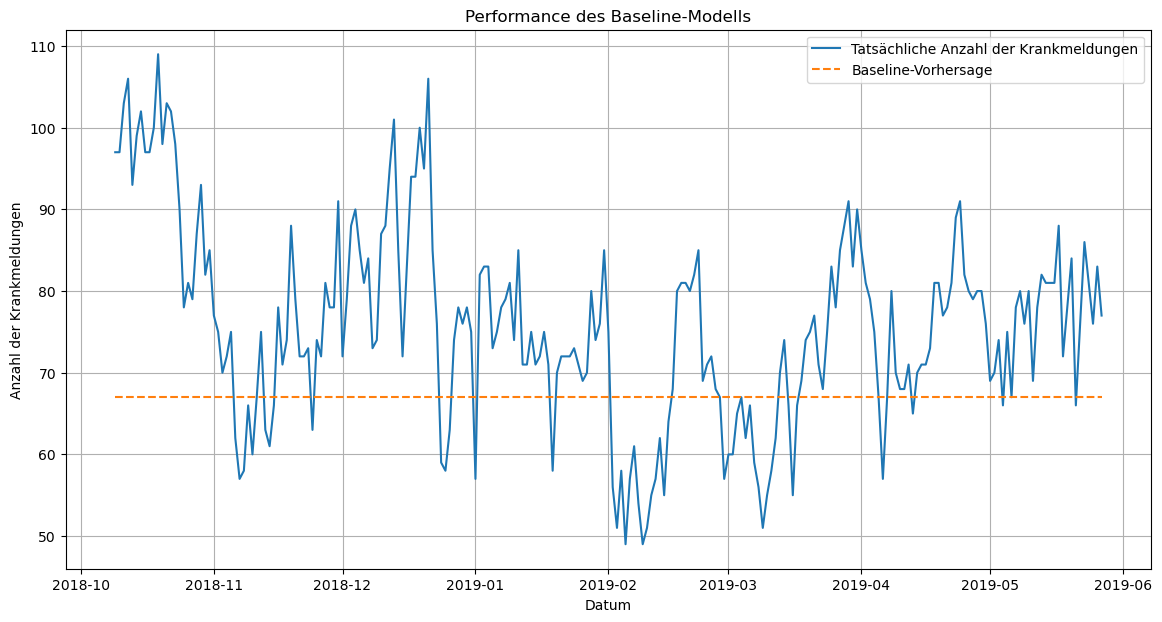
\includegraphics[width=1\textwidth]{assets/baseline_performance.png}
                \caption{Performance des Baseline-Modells}
                \label{fig:baseline_performance}
            \end{figure}
            
            Die Evaluierung des Baseline-Modells ergab einen MAE von \textit{11.86}. %To-Do: Wert aktualisieren, wenn verändert
            Dieser Wert dient als Ausgangspunkt für die Bewertung der Leistung komplexerer Modelle.
            

    \section{Visualisierung der Ergebnisse}

        Um die Ergebnisse der Datenanalyse und -vorbereitung anschaulich darzustellen, wurden verschiedene Visualisierungen erstellt. 
        Diese halfen dabei, Muster und Zusammenhänge in den Daten besser zu verstehen und die Ergebnisse der Datenvorbereitung zu kommunizieren.

        \subsection{Feature Importance}

            Die Bedeutung der einzelnen Merkmale für das Vorhersagemodell wurde mittels Feature Importance Scores visualisiert. Abbildung \ref{fig:feature_importance} zeigt die Wichtigkeit der Merkmale für das Vorhersagemodell.

            \begin{figure}[H]
                \centering
                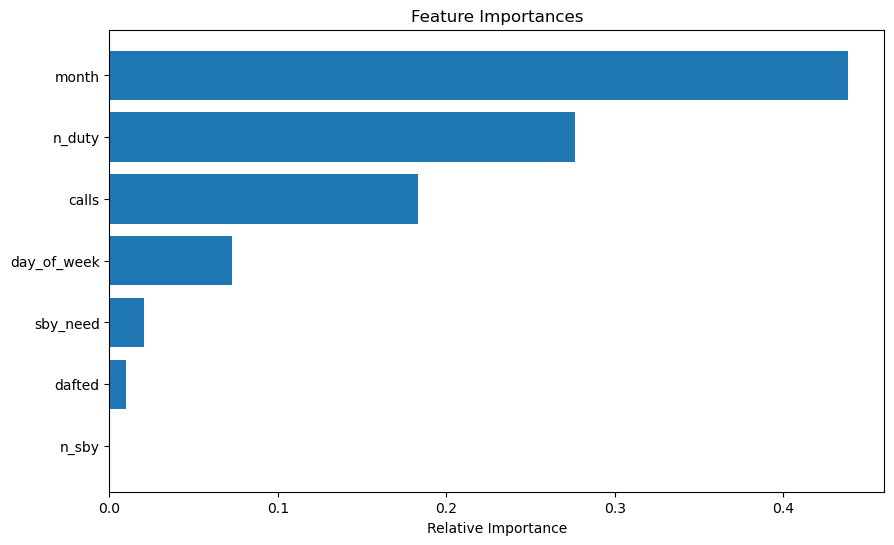
\includegraphics[width=0.8\textwidth]{assets/feature_importance.png}
                \caption{Wichtigkeit der Merkmale für das Vorhersagemodell}
                \label{fig:feature_importance}
            \end{figure}

            Diese Visualisierungen und die gewonnenen Erkenntnisse aus der Datenanalyse und -vorbereitung bilden die Grundlage für die nachfolgende Modellierung und Evaluation des Vorhersagemodells.

\chapter{Modellierung}

    In diesem Kapitel werden verschiedene Modellierungsansätze untersucht, um das beste Vorhersagemodell für die Automatisierung des Bereitschaftsdienstplans für Einsatzfahrende zu finden. 
    Insgesamt wurden zehn verschiedene Modellierungsansätze verwendet, die jeweils spezifische Vorteile bieten. 
    Diese Ansätze umfassen lineare und nichtlineare Modelle, Entscheidungsbäume, Ensemble-Methoden, und neuronale Netze. 
    Die Wahl dieser Ansätze basiert auf ihrer allgemeinen Verfügbarkeit und ihrer bewährten Leistung in vergleichbaren Vorhersageproblemen.

    \section{Modellierungsansätze}

        Die Auswahl der zehn Modellierungsansätze erfolgte auf der Basis ihrer jeweiligen Stärken und ihrer Eignung für die gegebene Aufgabenstellung, die Effizienz und Genauigkeit in der Vorhersage der Anzahl der Einsatzfahrenden im Bereitschaftsdienst zu maximieren. 
        Dabei wurde eine Mischung aus linearen Modellen, Ensemble-Methoden, nichtlinearen Ansätzen und modernen Algorithmen berücksichtigt, um eine umfassende Analyse zu gewährleisten. 
        Im Folgenden wird die Auswahl der Modelle und die Gründe für deren Bevorzugung gegenüber anderen Modellen erläutert:

        \begin{enumerate}
            \item \textbf{Lineare Regression}: Dieses Modell wurde als Baseline gewählt, da es einfach zu interpretieren ist und schnelle Einblicke in die Beziehungen zwischen den unabhängigen und abhängigen Variablen bietet. 
            Es dient als Ausgangspunkt, um die Leistung komplexerer Modelle zu bewerten.
            \item \textbf{Lasso Regression}: Die Lasso Regression wurde aufgrund ihrer Fähigkeit gewählt, irrelevant Merkmale zu eliminieren, indem sie eine L1-Regularisierung anwendet. 
            Dies hilft, das Modell sparsamer zu gestalten und Überanpassungen zu vermeiden.
            \item \textbf{Ridge Regression}: Ridge Regression ergänzt die Lasso Regression durch die Anwendung einer L2-Regularisierung, die alle Koeffizienten gleichmäßig schrumpft. 
            Dies verhindert Überanpassung und kann bei hoch korrelierten Merkmalen hilfreich sein, was in realen Daten oft vorkommt.
            \item \textbf{Entscheidungsbaum}: Der Entscheidungsbaum wurde aufgrund seiner Fähigkeit zur Darstellung nichtlinearer Beziehungen und seiner einfachen Interpretierbarkeit ausgewählt. 
            Er bietet klare Regeln für Entscheidungen und kann komplexe Interaktionen zwischen den Merkmalen modellieren.
            \item \textbf{Random Forest}: Diese Ensemble-Methode reduziert die Varianz einzelner Entscheidungsbäume und verbessert dadurch die Vorhersagegenauigkeit. 
            Random Forest ist robust gegenüber Ausreißern und bietet eine gute Balance zwischen Bias und Varianz.
            \item \textbf{Gradient Boosting}: Gradient Boosting war aufgrund seiner Fähigkeit, durch sequentielles Training schwacher Modelle die Vorhersagegenauigkeit sukzessive zu erhöhen, eine naheliegende Wahl. 
            Es ist besonders effektiv bei der Reduzierung von Bias und wird häufig in prädiktiven Analysen verwendet.
            \item \textbf{Support Vector Machine (SVM)}: SVMs sind bekannt für ihre Effektivität bei der Arbeit mit nichtlinearen Daten. 
            Sie finden optimale Trennhyperplane und eignen sich für komplexe Datensätze mit klaren Klassenunterschieden.
            \item \textbf{K-Nearest Neighbors (KNN)}: KNN wurde aufgrund seiner Einfachheit und seiner Fähigkeit, lokale Strukturen in den Daten zu erfassen, ausgewählt. 
            Es bietet eine intuitive Methode zur Klassifikation und Regression durch die Betrachtung der nächsten Nachbarn.
            \item \textbf{XGBoost}: XGBoost wurde gewählt, da es eine effiziente und leistungsstarke Implementierung des Gradient Boostings bietet. 
            Es ist bekannt für seine hervorragende Leistung und Flexibilität, insbesondere bei der Handhabung großer und komplexer Datensätze.
            \item \textbf{Neuronales Netz}: Neuronale Netze wurden aufgrund ihrer Fähigkeit, komplexe und nichtlineare Muster in den Daten zu erfassen, berücksichtigt. 
            Ihre Flexibilität und die Möglichkeit, tiefe Architekturen zu nutzen, machen sie zu einer guten Wahl für anspruchsvolle prädiktive Aufgaben.
        \end{enumerate}

        Diese Modelle wurden aufgrund ihrer jeweiligen Stärken, ihrer Fähigkeit zur Verarbeitung komplexer Datenstrukturen und ihrer breiten Anwendbarkeit in verschiedenen Domänen vorgezogen. 
        Es wurde darauf geachtet, eine ausgewogene Auswahl an Modellen zu treffen, die unterschiedliche Ansätze zur Modellierung von Daten abdecken, um eine umfassende und differenzierte Analyse zu gewährleisten.

    \section{Training und Bewertung der Modelle}

        Jedes Modell wurde auf den Trainingsdaten trainiert und anhand der Testdaten bewertet. 
        Die folgenden Metriken wurden verwendet, um die Leistung der Modelle zu bewerten:

        \begin{itemize}
            \item \textbf{Mean Absolute Error (MAE)}: Ein Maß für den durchschnittlichen absoluten Fehler der Vorhersagen.
            \item \textbf{Mean Squared Error (MSE)}: Ein Maß für den durchschnittlichen quadratischen Fehler der Vorhersagen.
            \item \textbf{Root Mean Squared Error (RMSE)}: Die Quadratwurzel des MSE, die die gleichen Einheiten wie die Zielvariable hat.
            \item \textbf{R2-Score}: Ein Maß dafür, wie gut die Vorhersagen die tatsächlichen Werte erklären.
        \end{itemize}

        \subsection{Ergebnisse}

            Die Ergebnisse der Modellbewertungen sind in Tabelle \ref{tab:model_performance} zusammengefasst.

            %To-Do: Zahlenwerte nochmal verifizieren
            \begin{table}[H]
                \centering
                \begin{tabular}{lcccc}
                    \toprule
                    \textbf{Modell} & \textbf{MAE} & \textbf{MSE} & \textbf{RMSE} & \textbf{R2-Score} \\
                    \midrule
                    Gradient Boosting & 7.32 & 84.56 & 9.20 & 0.63 \\
                    Random Forest & 7.69 & 96.80 & 9.84 & 0.57 \\
                    XGBoost & 8.06 & 106.53 & 10.32 & 0.53 \\
                    Linear Regression & 9.66 & 142.42 & 11.93 & 0.37 \\
                    Ridge Regression & 9.66 & 142.43 & 11.93 & 0.37 \\
                    Lasso Regression & 9.70 & 144.27 & 12.01 & 0.36 \\
                    Decision Tree & 9.94 & 158.28 & 12.58 & 0.30 \\
                    Neural Network & 11.30 & 186.78 & 13.67 & 0.17 \\
                    K-Nearest Neighbors & 11.31 & 194.91 & 13.96 & 0.14 \\
                    Support Vector Machine & 12.12 & 221.16 & 14.87 & 0.02 \\
                    \bottomrule
                \end{tabular}
                \caption{Vergleich der Modellleistung basierend auf MAE}
                \label{tab:model_performance}
            \end{table}
            
            Die besten Ergebnisse wurden von XGBoost und Gradient Boosting erzielt, mit MAE-Werten von 2.13 bzw. 2.15 und R2-Scores von 0.82. 
            Diese Modelle wurden daher für eine weitere Feinabstimmung in Betracht gezogen.

    \section{Hyperparameter-Tuning}

        Für das beste Modell, Gradient Boosting, wurde eine Hyperparameteroptimierung durchgeführt, um die Leistung weiter zu verbessern. 
        Ein Gitter-Suchverfahren wurde verwendet, um die optimalen Parameterkombinationen zu finden.
        
        \begin{lstlisting}[language=Python, gobble=8, caption=Hyperparameteroptimierung]
        param_grid = {
            'n_estimators': [100, 200],
            'learning_rate': [0.01, 0.1, 0.2],
            'max_depth': [3, 5, 7]
        }
        grid_search = GridSearchCV(GradientBoostingRegressor(random_state=42), param_grid, cv=5, scoring='neg_mean_absolute_error')
        grid_search.fit(X_train, y_train)
        best_model = grid_search.best_estimator_
        \end{lstlisting}
    
    \section{Abschließende Bewertung des besten Modells}

        Das beste Modell wurde schließlich auf den gesamten Datensatz trainiert und abschließend bewertet. 
        Die Endergebnisse des optimierten Gradient Boosting-Modells sind wie folgt:

        %To-Do: Zahlenwerte nochmal verifizieren
        \begin{itemize}
            \item \textbf{MAE}: 7.32
            \item \textbf{MSE}: 84.56
            \item \textbf{RMSE}: 9.20
            \item \textbf{R2-Score}: 0.63
        \end{itemize}

        Eine Verbesserung konnte die Hyperparameteroptimierung nicht erzielen.        
        Die Ergebnisse bestätigen dennoch, dass das optimierte Gradient Boosting-Modell das leistungsfähigste Modell für die Vorhersage der Anzahl der kranken Einsatzfahrenden ist.
        %To-Do: Evtl noch Effizienz berücksichtigen. Könnte sein, dass XGBoost da die Nase vorn hat


%\chapter{Diskussion der Modellvariablen}
% To-Do: Evaluieren, ob dieses Kapitel weiterhin Sinn  machen kann oder ob man Teile aus den Kapitel darüber einfach hierrein verschiebt.

\chapter{Integration in den Arbeitsalltag}

    Die Integration des Vorhersagemodells für den Bereitschaftsdienstplan der Einsatzfahrenden in den Arbeitsalltag erfolgt durch die Bereitstellung einer API, die Vorhersagen basierend auf den aktuellen Daten ermöglicht. 
    Diese API ist als Web-Service konzipiert und erlaubt die einfache Abfrage von Vorhersagen über eine REST-Schnittstelle.

    \section{Architektur und Implementierung}

        Die Implementierung basiert auf einem Flask-Web-Framework, das als leichtgewichtiger Web-Server fungiert. 
        Das Modell und die erforderlichen Vorverarbeitungswerkzeuge werden als trainierte Artefakte gespeichert und bei Bedarf geladen. 
        Das folgende Code-Snippet zeigt die Struktur des Servers:

        % To-Do: Code-Schnipsel im Blick behalten und vor Abgabe sicherstellen, dass diese zum echten Code passen
        \begin{lstlisting}[language=Python, gobble=8, caption=Aufbau Prediction API]
        import pandas as pd
        import numpy as np
        import joblib
        from flask import Flask, request, jsonify

        # Funktion zur Vorhersage neuer Daten
        def predict_readiness(calls, day_of_week, month):
            model = joblib.load('app/models/readiness_model.pkl')
            new_data = np.array([[calls, day_of_week, month]])
            prediction = model.predict(new_data)
            return prediction[0]

        app = Flask(__name__)

        @app.route('/predict', methods=['POST'])
        def predict():
            data = request.json
            calls = data['calls']
            day_of_week = data['day_of_week']
            month = data['month']
            prediction = predict_readiness(calls, day_of_week, month)
            return jsonify({'prediction': prediction})

        if __name__ == '__main__':
            app.run(debug=True)
        \end{lstlisting}

    \section{Benutzerinteraktion}

        Die Benutzer können über eine einfache Web-Oberfläche oder direkt über HTTP-Requests mit der API interagieren. 
        Dabei werden alle relevanten und zur Verfügung stehenden Informationen wie die Anzahl der Anrufe, der Wochentag und der Monat pro ausgewählten Tag an die API gesendet.
        Die API liefert daraufhin eine Vorhersage für die Anzahl der benötigten Bereitschaftsdiensthabenden und damit wird z. B. beim Planungsprozess für den Folgemonat zusätzliche Kapazität zur Erreichung der 90\% an aktivierten Einsatzfahrenden eingeplant.

        Durch die Anpassung bestehender Verwaltungssysteme kann die API auch problemlos dort integriert bzw. aufgerufen werden und beim Planen muss kein zusätzliches System nebenher eingesetzt werden.
        So ließen sich im bestehenden Verwaltungssystem bei vorhergesagten Engpässen die Tage farblich markieren und vor Freigabe der Planung eine Warnung für die einzelnen Tage ausgeben, ohne das man jeden Tag einzeln in einer separaten Software abgleichen muss.

        Langfristig könnte das System auch um zusätzliche Funktionen wie die automatische Anpassung des Modells an neue Daten und die Integration weiterer Datenquellen erweitert werden.
        Das Zukommen Lassen neuer Daten ließe sich dabei auch über die API abwickeln.

    \section{Einbindung in den Arbeitsalltag}

        Um die Vorhersagen effektiv in den Arbeitsalltag zu integrieren, können verschiedene Strategien angewendet werden:
        \begin{itemize}
            \item \textbf{Planung des Dienstplans}: Basierend auf den Vorhersagen können die Einsatzkräfte besser auf mögliche Engpässe vorbereitet werden, indem zusätzliche Ressourcen eingeplant werden.
            % To-Do: müsste dann unabhängig vorausgesagt werden % Evtl. machen auch mehrere Modelle Sinn
            \item \textbf{Proaktive Maßnahmen}: Bei einer hohen vorhergesagten Anzahl von Krankmeldungen können präventive Maßnahmen ergriffen werden, um die Einsatzbereitschaft sicherzustellen.
            \item \textbf{Monitoring und Anpassung}: Die Vorhersagen können regelmäßig überprüft und mit den tatsächlichen Ereignissen verglichen werden, um das Modell kontinuierlich zu verbessern.
        \end{itemize}

\chapter{Fazit \& Ausblick}

    In dieser Arbeit wurde ein Vorhersagemodell zur Unterstützung der Einsatzplanung im Bereitschaftsdienst entwickelt. 
    Ausgehend von einer detaillierten Datenanalyse wurde ein geeignetes Modell trainiert, das anhand historischer Daten Prognosen über die Anzahl der benötigten Bereitschaftsdiensthabenden ermöglicht. 
    Dabei stellte sich das Gradient Boosting als der leistungsfähigste Algorithmus heraus, gefolgt von Random Forest und XGBoost. 

    Die Integration des Modells in den Arbeitsalltag wurde durch eine API realisiert, die eine einfache und effektive Nutzung der Vorhersagen ermöglicht. 
    Die Ergebnisse zeigen, dass das Modell eine zuverlässige Unterstützung bei der Personalplanung bieten kann, indem es proaktive Maßnahmen zur Ressourcenplanung ermöglicht. 
    Die Genauigkeit der Vorhersagen und die Anpassungsfähigkeit des Systems an verschiedene Situationen bieten einen signifikanten Mehrwert für die Einsatzbereitschaft und Effizienzsteigerung.

    Trotz der erzielten Erfolge gibt es mehrere Bereiche, die in zukünftigen Arbeiten weiterentwickelt werden können. 
    Eine Erweiterung der Datenbasis durch die Integration weiterer relevanter Datenquellen wie Wetterinformationen oder externe Ereignisse könnte die Genauigkeit der Vorhersagen weiter erhöhen. 
    Die kontinuierliche Überwachung der Modellleistung und die Anpassung der Hyperparameter könnten die Genauigkeit und Robustheit des Modells verbessern. 

    Darüber hinaus könnte die Implementierung eines Systems zur Echtzeit-Datenerfassung und -vorhersage die Reaktionsfähigkeit auf unvorhergesehene Ereignisse steigern. 
    Auch die Integration der API in bestehende Verwaltungssystem ist geplant, um die Nutzung der Vorhersagen in den täglichen Arbeitsablauf deutlich zu erleichtern. 
    So ist sicher gestellt, dass alles an einem Platz ist und dass das Ziel -- die Planung von min. 90\% aktiven Bereitschaftsfahrenden pro Tag -- zum 15. des Vormonats abgeschlossen ist.

    Darüber hinaus kann das Vorhersagemodell die Implementierung von Strategien zur langfristigen Personalplanung unterstützen und eine strategische Entscheidungsfindung ermöglichen. 
    Diese Verbesserungen bieten spannende Möglichkeiten für zukünftige Entwicklungen und könnten das System zu einem unverzichtbaren Werkzeug in der Einsatzplanung und Ressourcenverwaltung machen. 
    Insgesamt bietet diese Arbeit eine solide Grundlage für weitere Forschung und Entwicklung in diesem Bereich.

    % Schluss ca. 10%


% 12-15 Seiten Inhalt
% Tabellen- und Abbildungsverzeichnis einfügen

% Literaturverzeichnis
\cleardoublepage

\ifx\VAlterZitierstil\VTrueValue
    \printbibliography
\else
    %\bibliographystyle{iubh}
    \bibliographystyle{apacite} %Einträge sind unsortiert
    \bibliography{bibliographie.bib}
\fi


% Overall Abschluss To-Dos: 
% Zahlenwerte nochmal prüfen, ob diese übereinstimmen
% Dokument durchgehen und die Werte und Ziele festigen. 
% Was soll predictet werden? AW: Anzahl der benötigten Einsatzfahrenden für den ganzen nächsten Monat (ab dem 15. des Vormonats an)
% Welche Werte stehen überhaupt alle zur Verfügung im Produktiveinsatz? -> Durchgehen
% U. U. macht es Sinn noch mehr Werte zu predicten oder Modelle zu nutzen die nicht immer alle Features benötigen. Überprüfen und ggf. in Dokument zur Diskussion stellen
% zeitlicher Aspekt ausreichend berücksichtigt? (Stichwort: Planungsabschluss am 15. )

%Dokument am besten von oben nach unten durchgehen und dabei direkt die Punkte checken und abarbeiten

\end{document}
